\chapter{Endoscopic Image Classification with Symptom-Localization \&  Data Augmentation}
%Proposed methods for abnormality finding and landmark detection for endoscopic images
\label{chap-method-endoscopy}
\begin{ChapAbstract}
In this chapter, we present our proposed method for abnormal finding and landmark detection in endoscopic images. Particularly, our proposed methods are used to take part in two challenges, including the Medico: The 2018 Multimedia for Medicine Task (Medico 2018) and The Biomedia ACM MM Grand Challenge 2019 (Biomedia 2019). Details about our approaches and improvements between two challenges are also reported. In sum, We utilize different  deep convolution neural network architectures together with several training techniques to improve the overall performance.
\end{ChapAbstract}

\section{Overview of proposed methods}
To tackle with the image classification problem, we consider using a stacked model consisting of two deep networks, a Residual Neural Network (ResNet) followed by a Faster Region-based Convolutional Neural Network (FasterR-CNN). We carefully analyze the results after each intermediate steps to understand about the properties of each module. As our observation, the image classification already proposed significant results in term of the accuracy on our validation set. However, it fails to classify images that abnormal symptoms of diseases or instruments appeared as  small objects on diversity backgrounds. It happens because of the ResNet mostly focuses on deep global features of image, when we just feed all of them into the network. Therefore, this is the reason of using Faster R-CNN to re-classify the images of some classes that ResNet usually mis-classifies. 

Nevertheless, inference time must be taken into account, while the Faster R-CNN needs longer time to process than that of ResNet. Therefore, instead of feeding all images through the ResNet module, we should have a strategy that reduce the number of images need to go through the Faster R-CNN module. We propose several configurations as our official submissions, as presented in Section \ref{5runs_config}.

Besides, due to the diversity of endoscopic images, various kind of abnormalities can appear in one image, that image can be classified into multiple classes simultaneously. Regarding to this  Multi-class classification problem, the task organizers of the Medico 2018 propose a priority list which forces every systems of participants should return only one class which has the most important level compare to others. In Medico 2018, we tried to force our model by re-organize the training set together with adding extra training samples in order to help our model can learn that priority list. However, we found out that it is also possible to propose a multi-task classification architecture that can predict multiple classes at the same time, which can reduce the confusing level of the image classifier model in these difficult cases. Further information about this architecture is presented in Section \ref{sec:multi_task}.
 
In the development dataset, there is an unbalance between classes and false labeling which are commonly occurred in medical dataset. Unbalancing between classes can make deep models bias to some classes than others, which reduce the overall accuracy. Moreover, one of the goals of these challenge is using as less as training data as possible, therefore, using extra data from other dataset is not possible in this case. Nevertheless, in order to build the object detection model as we mentioned before, extra information about the location of symptoms must be given, i.e bounding boxes can be used to localize these locations. Regarding to mentioned problems, in this work, besides annotating symptoms of diseases which is described in Section \ref{sec:symptoms_local}, we also provide some augmentation mechanism on the given training dataset in order to provide a better version for the training step of both Faster R-CNN module and ResNet module. See Section \ref{sec:augment} a complete description of our work related to our data augmentation strategy.  

\section{From Classification to Symptoms Region Localization}
\label{sec:symptoms_local}
Obviously, to enhance the performance of our system, an object detection module can be really useful to detect small abnormal symptoms and diseases, such as \textit{polyps, instruments, dyed-lifted-polyps} and \textit{dyed-resection-margins}. Besides, in some cases that multi-symptoms appear in the same image, identify all of them is necessary to draw the final conclusion. Nevertheless, system that can not only predict the abnormalities but also propose the corresponding positions of that is more reliable and more convenient for endoscopists. Estimating the sizes of these abnormalities can  become really efficient for future systems. 

In order to train an object detection model, besides an images dataset, we also need the corresponding bounding boxes for each abnormality and passed them to the model as input during the training phase. 

Due to the limitation of the given training dataset, there is no extra information about positions of abnormalities inside image  given. Therefore, in our first step, we decided to annotate all the abnormal symptoms in every images of the following classes: \textit{dyed-resection-margins, dyed-lifted-polyps, instruments} and \textit{polyps} with the help of the LabelImg \footnote{\url{https://github.com/tzutalin/labelImg}} annotation tool. Examples of our proposed bounding box can be seen in Figure \ref{fig:symptoms_localization}.

\begin{figure}[thb]
\begin{center}
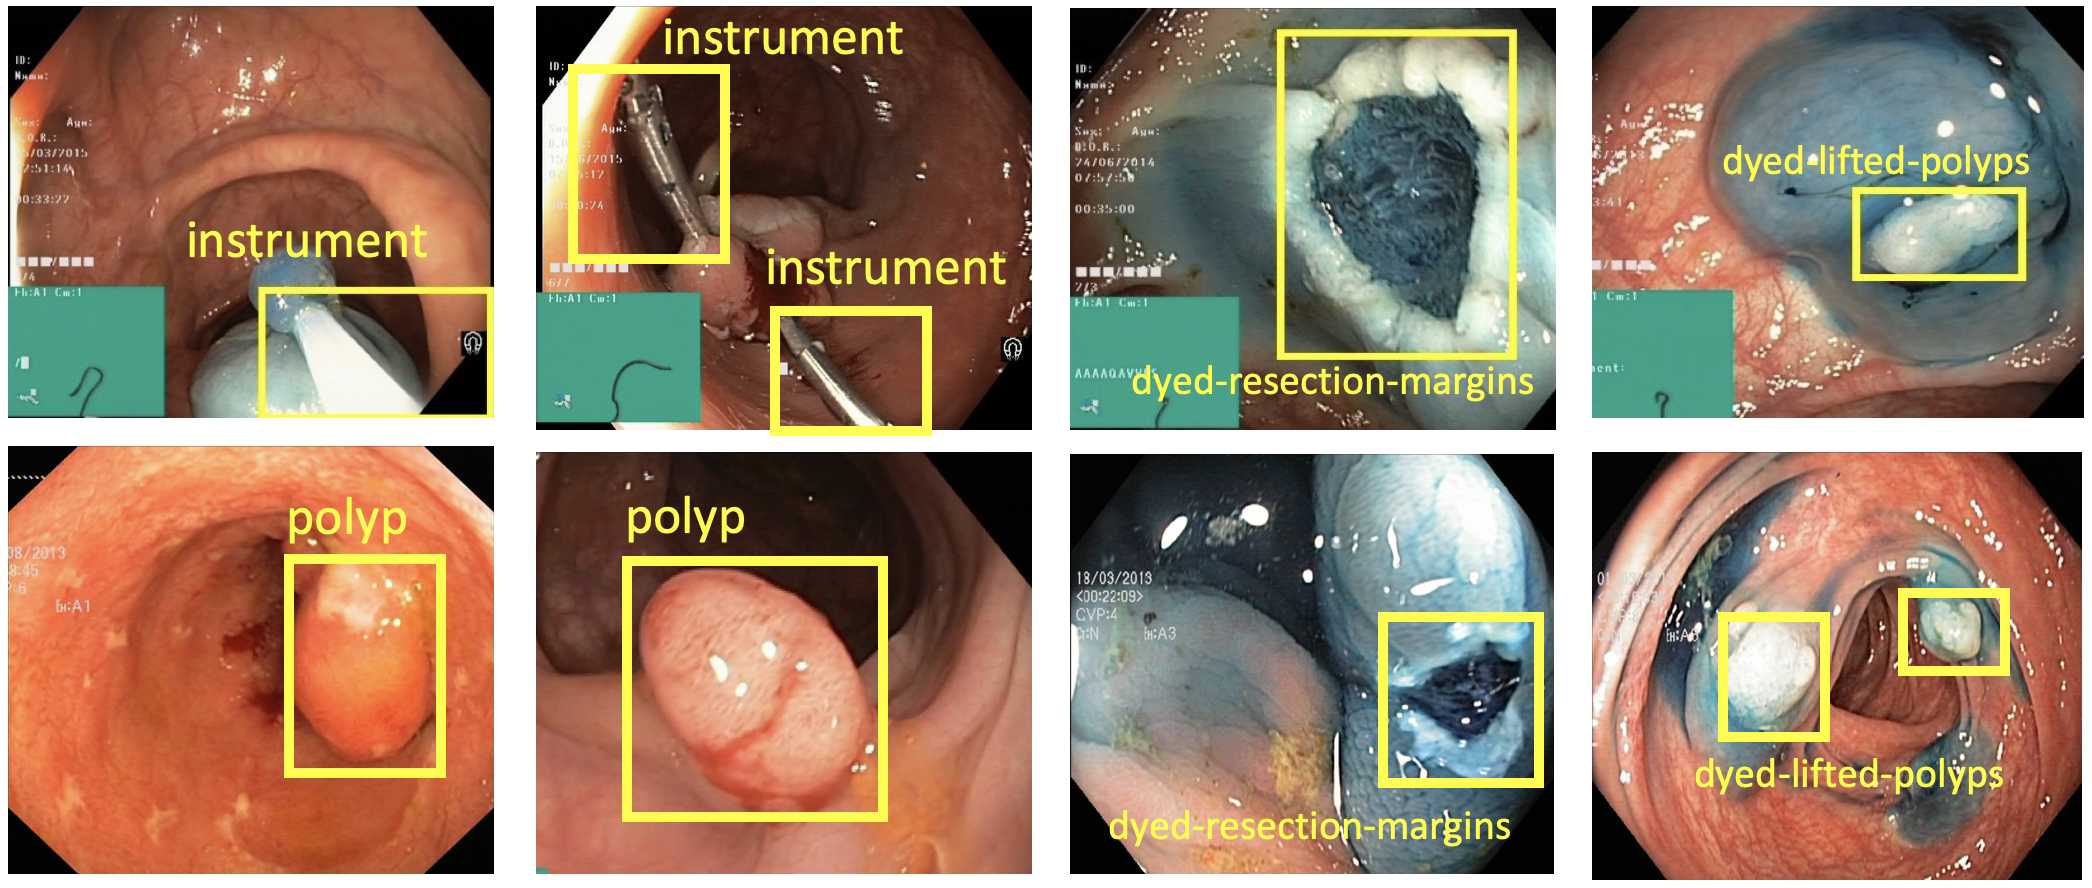
\includegraphics[width=\textwidth]{endoscopy_resources/symptoms_region_localization.png}
\end{center}
   \caption{Our proposed symptoms region localization, annotated images with corresponding bounding boxes and classes name.}
\label{fig:symptoms_localization}
\end{figure}

Totally, with 5241 images belong to the following classes: \textit{polyp, dyed-lifted-polyp, dyed-resection-margins} and \textit{instruments} category are annotated with 5715 bounding boxes from the Kvasir dataset \cite{Pogorelov:2017:KMI:3083187.3083212} and Medico 2018 development dataset. The number of bounding boxes for each class is reported in Table \ref{tab:count_bbox}. Although, the number of training samples we annotated is much larger than the number of actual training samples we used in training phase, it is still useful for future works. 

\begin{table}[tbh]
\caption{Number of annotated bounding boxes from each class.}
\centering
\begin{tabular}{|l|c|}
\hline
\multicolumn{1}{|c|}{\textbf{Class}} & \textbf{Number of bounding boxes} \\ \hline
\textit{dyed-lifted-polyp}                    & 1513                              \\ \hline
\textit{dyed-resection-margin}                & 1509                              \\ \hline
\textit{polyp}                                & 2657                              \\ \hline
\textit{instruments}                          & 36                                \\ \hline
\multicolumn{1}{|c|}{Total}          & 5715                              \\ \hline
\end{tabular}
\label{tab:count_bbox}
\end{table}

\section{Addition Labeling for \textit{Instruments} versus Other Classes}
As our viewpoint, the \textit{instruments} and \textit{polyps} are classes that are likely to appear together with other classes. We decided to annotated and mark every image in the development dataset which contains \textit{instruments}/\textit{polyps} or not. These addition labels are useful for us to train the Multi-task classification network which is further described in Section \ref{sec:multi_task}.

\section{Instruments Dataset Augmentation}
\label{sec:augment}
\textit{Instruments} - the second highest priority class has only 36 images with the limitation of background context in the Development set of Media Eval 2018. 

In order to maintain the balancing between all of these classes and also improve the diversity of the \textit{instruments} images, we aim to augment the given dataset by generate more images for the \textit{instruments} based on the current given development set by placing the instruments on the foreground of other diseases backgrounds.

Among the 36 \textit{instruments} images, we carefully select 24 of them and crop the instruments along their edges. Then, we randomly select images from \textit{dyed-lifted-polyps, dyed-resection-margins}, \textit{ulcerative-colitis} classes, and use them as the background of the cropped instruments. By applying this method, we are able to generate more than 800 images for the \textit{instruments} class. The overview of this process is illustrated in Figure \ref{fig:instruments_augment}.

\begin{figure}[thb]
\begin{center}
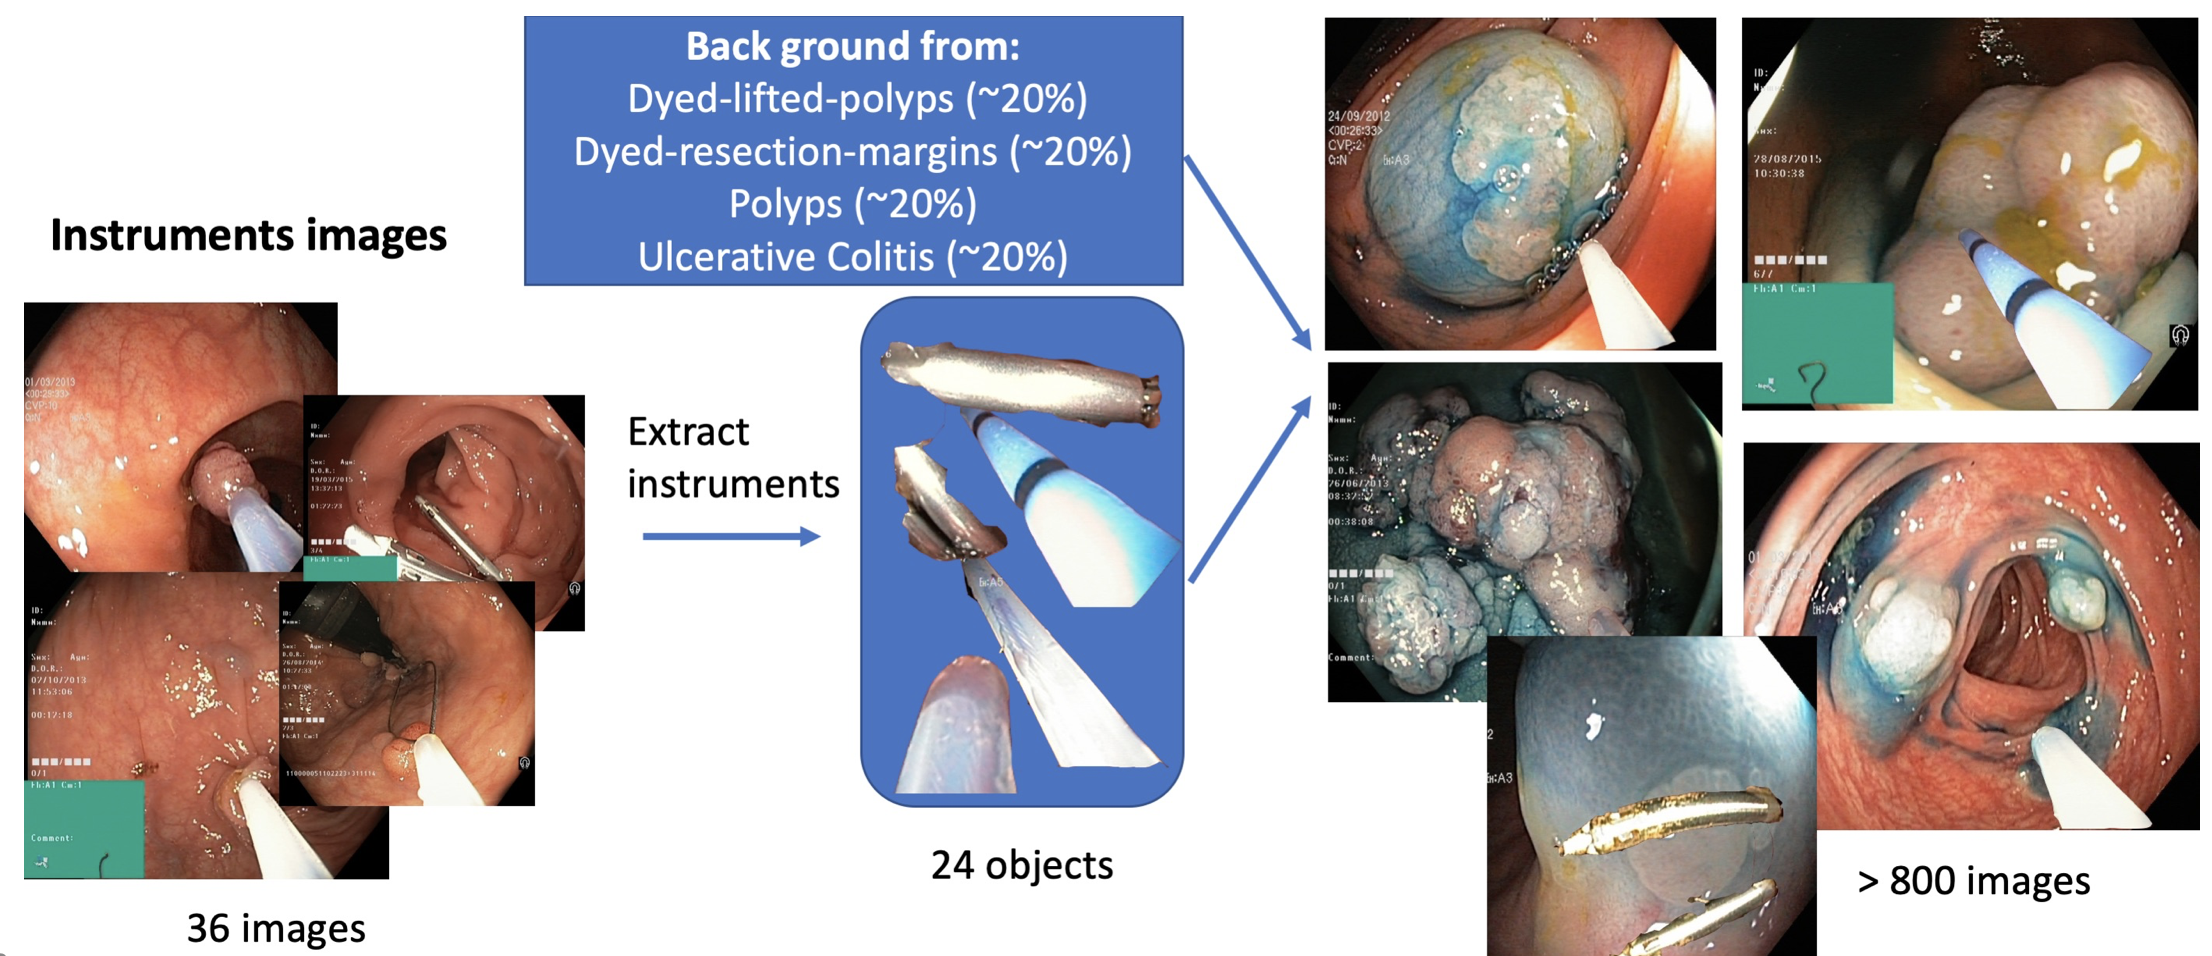
\includegraphics[width=\textwidth]{endoscopy_resources/instruments_augmentation.png}
\end{center}
   \caption{Overview of the \textit{Instruments} dataset augmentation process.}
\label{fig:instruments_augment}
\end{figure}

\begin{figure}[thb]
\begin{center}
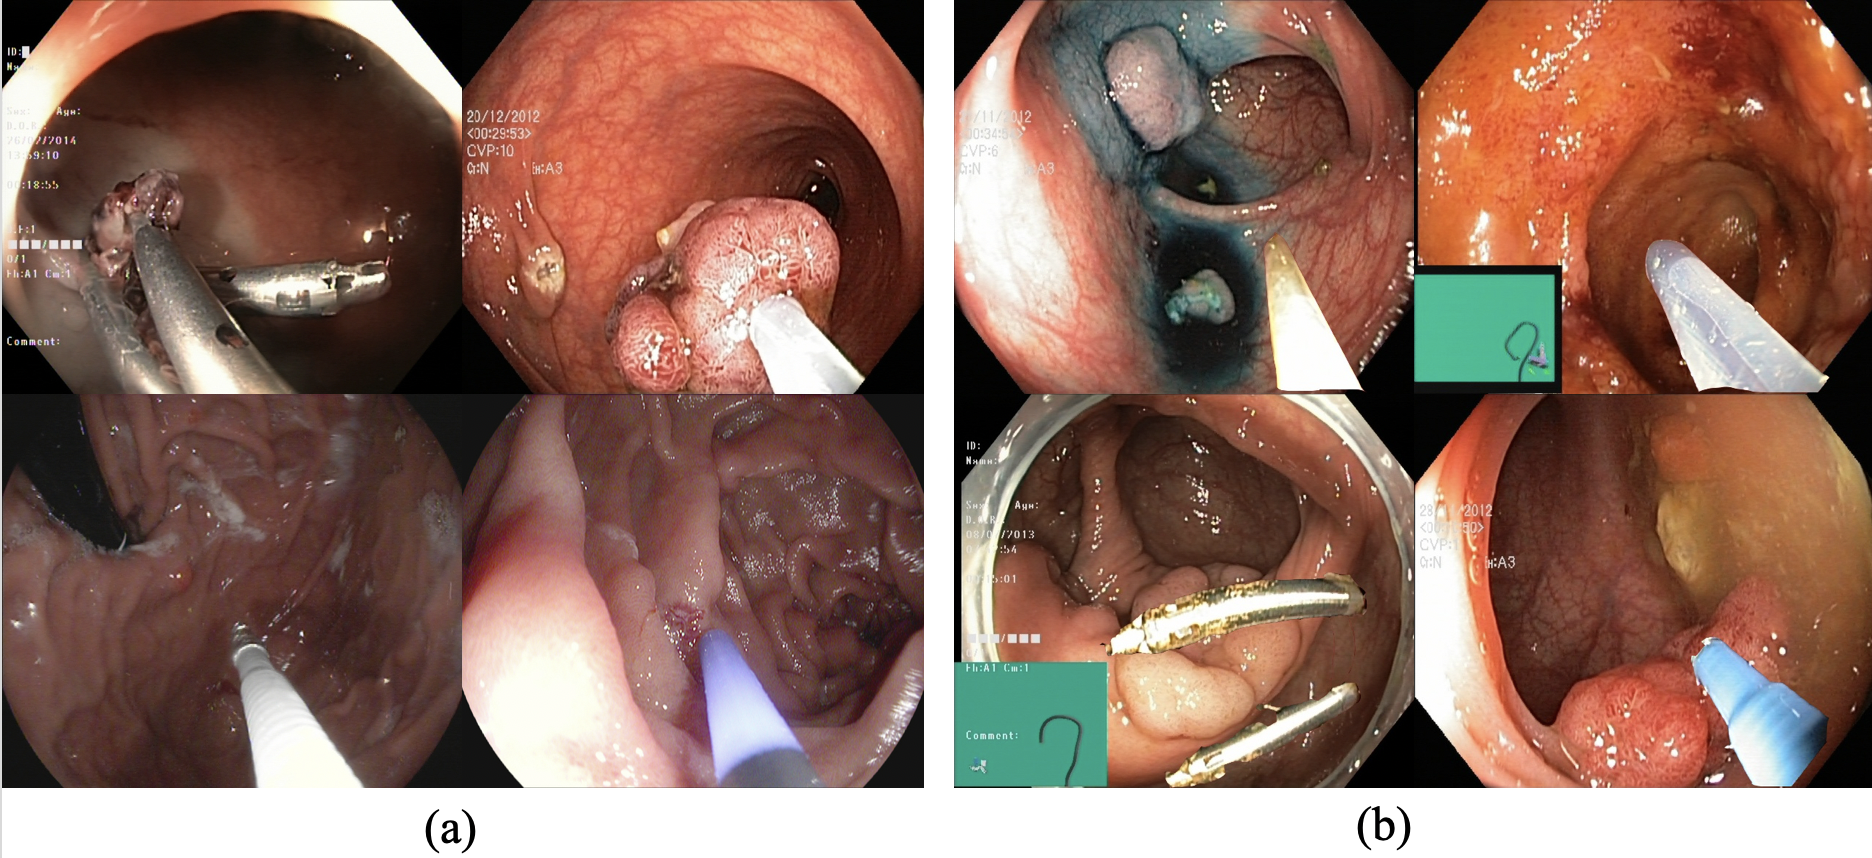
\includegraphics[width=\textwidth]{endoscopy_resources/instr_augment_compare.png}
\end{center}
   \caption{\textit{Instruments} dataset augmentation result. (a) original \textit{instruments} images in development dataset. (b) augmented \textit{instruments} images generated by our method}
\label{fig:instruments_augment_compare}
\end{figure}

\begin{figure}[thb]
\begin{center}
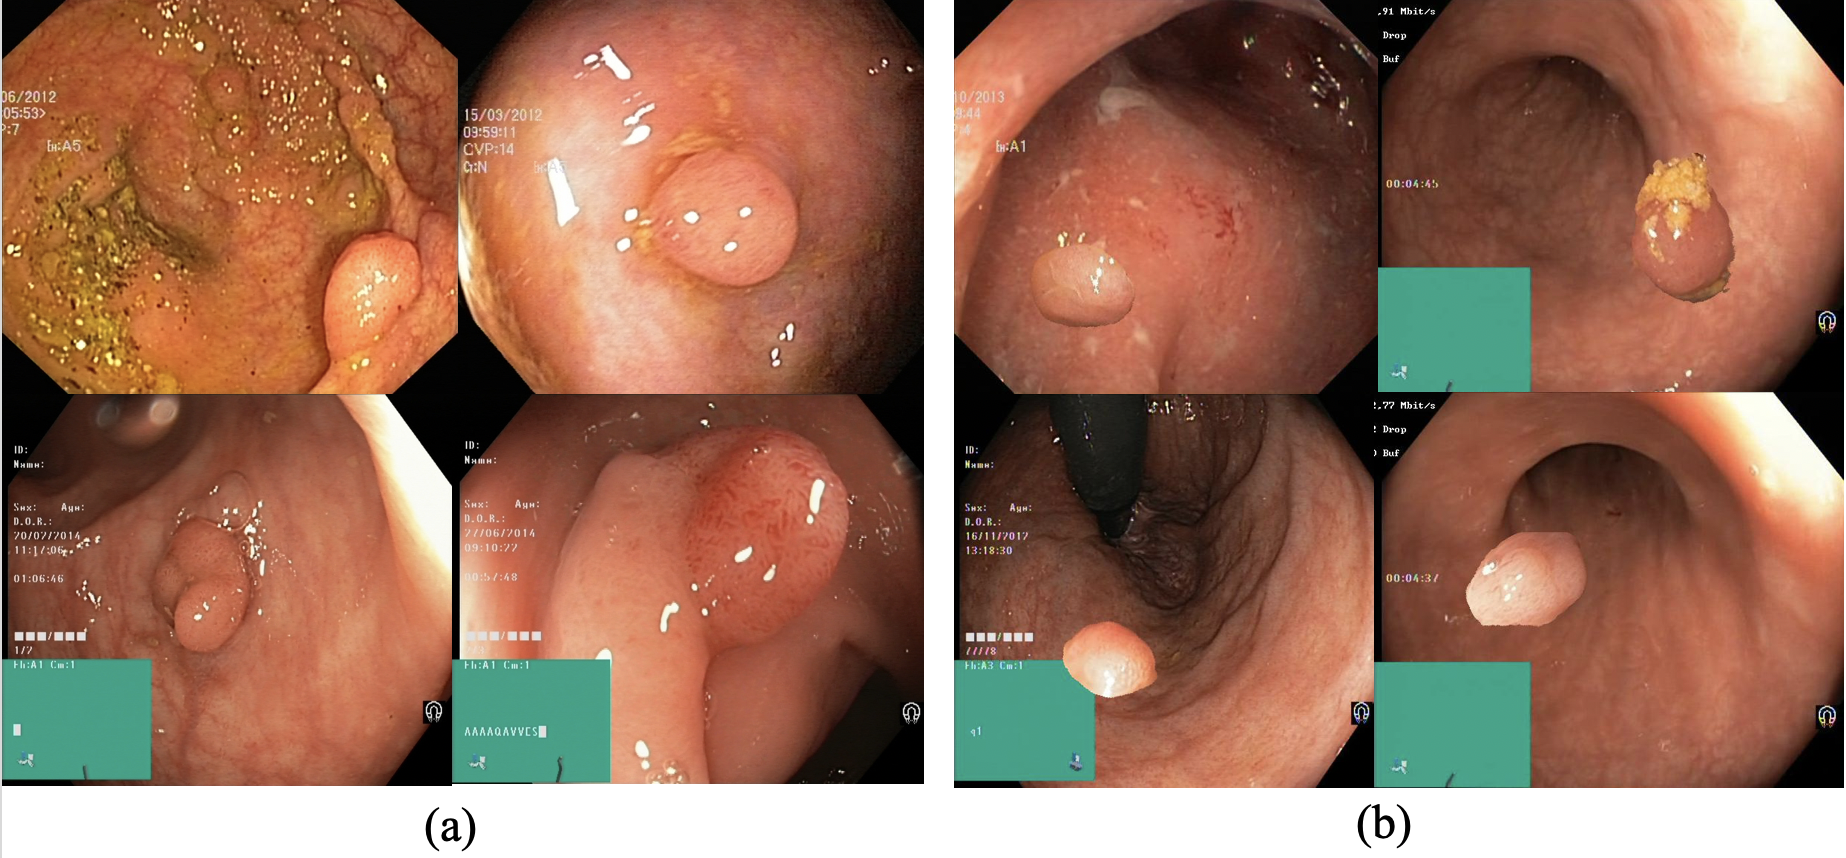
\includegraphics[width=\textwidth]{endoscopy_resources/polyp_augment_compare.png}
\end{center}
   \caption{\textit{Polyps} dataset augmentation result. (a) original \textit{polyps} images in development dataset. (b) augmented \textit{polyps} images generated by our method}
\label{fig:polyps_augment_compare}
\end{figure}

Figure \ref{fig:instruments_augment_compare} illustrates samples belong to the \textit{instruments} class, including  the  original samples and augmented samples. Similarly, Figure \ref{fig:polyps_augment_compare} demonstrates the augmentation result on the \textit{polyps} class. As our observation, there is not significant visual differences between samples from two groups. 

The augmented dataset can be used for both sub-task. By adding more positive examples to the training phase of the classification model, the performance of this model can be more robust. On the other hand, we  can easily get the position of the foreground object on generated images, which can be utilized to augment the training dataset of the objects detection module (Faster R-CNN). 

\section{Proposed system}
% 1) overview co re nhanh cac kieu
% 2) Mootj trong nhung cach endcode mot tam hinh, thay vi dung cai co san, dung 1 cai specialize , duoc dung  cho ca 2 task train end to end
% 3) Train Faster R-CNN 
\subsection{Overview}
Our approaches focus on utilizing the advantages of both object detection, such as Faster R-CNN and image classification, such as ResNet 101. However, due to the criterion of the endoscopy diagnosis system, the inference time of both modules must be taken into account. Noticeably, this number in Faster R-CNN is much larger than ResNet 101. By carefully observe the intermediate results of each module, we proposed several conditional strategies that limit the number of images feeding into the object detection module based on the  prediction  of image classification  module. In order to figure out the most balancing configuration for our method, multiple scenarios have been proposed and evaluate. Details about these configuration are presented in Section \ref{fig:5runs}.

\subsection{Fine-tuning Deep Neural Network on Endoscopic images}
Besides high computational cost, one of the main drawback of deep learning architecture is that it requires a large amount of training data. Moreover, labeled medical data
for supervised learning is limited and manual labelling of medical images is a difficult task. Therefore, it requires a lot of effort and time to train the network, which would depend on the size of training data used. However, there is a possible solution to deal with these limitations is
using transfer learning, where a pre-trained network on a large dataset (such as ImageNet \cite{ImageNet}) is used. 

In our approach, both Residual Network with 101 layers and Faster R-CNN \cite{chen17implementation} are both share a same features encoder. Therefore, it is necessary to propose a features encoder that is specialized on endoscopic images. This is the reason that we fine-tuned our deep neural network models (pre-trained on ImageNet) by using our modified development dataset. After training the whole neural network and then we freeze several first layers in its architecture and fine-tune the remains with small learning-rate. We also tried to train the network from scratch and all of our experiments point out that in term of using convolution neural network for medical images, knowledge transferring from natural images to medical images is possible, even though there is a large difference between the source and the target databases. 


This idea is also mentioned in \cite{trainingorfinetune}, it is especially useful in the case of small dataset of images provided. Fine-tuning on the ImageNet pre-trained model significantly improves the efficient of deep learning model on medical domains.

\section{Configuration of Conditional Scenarios}
\label{5runs_config}

\begin{figure}[tb!]
\begin{center}
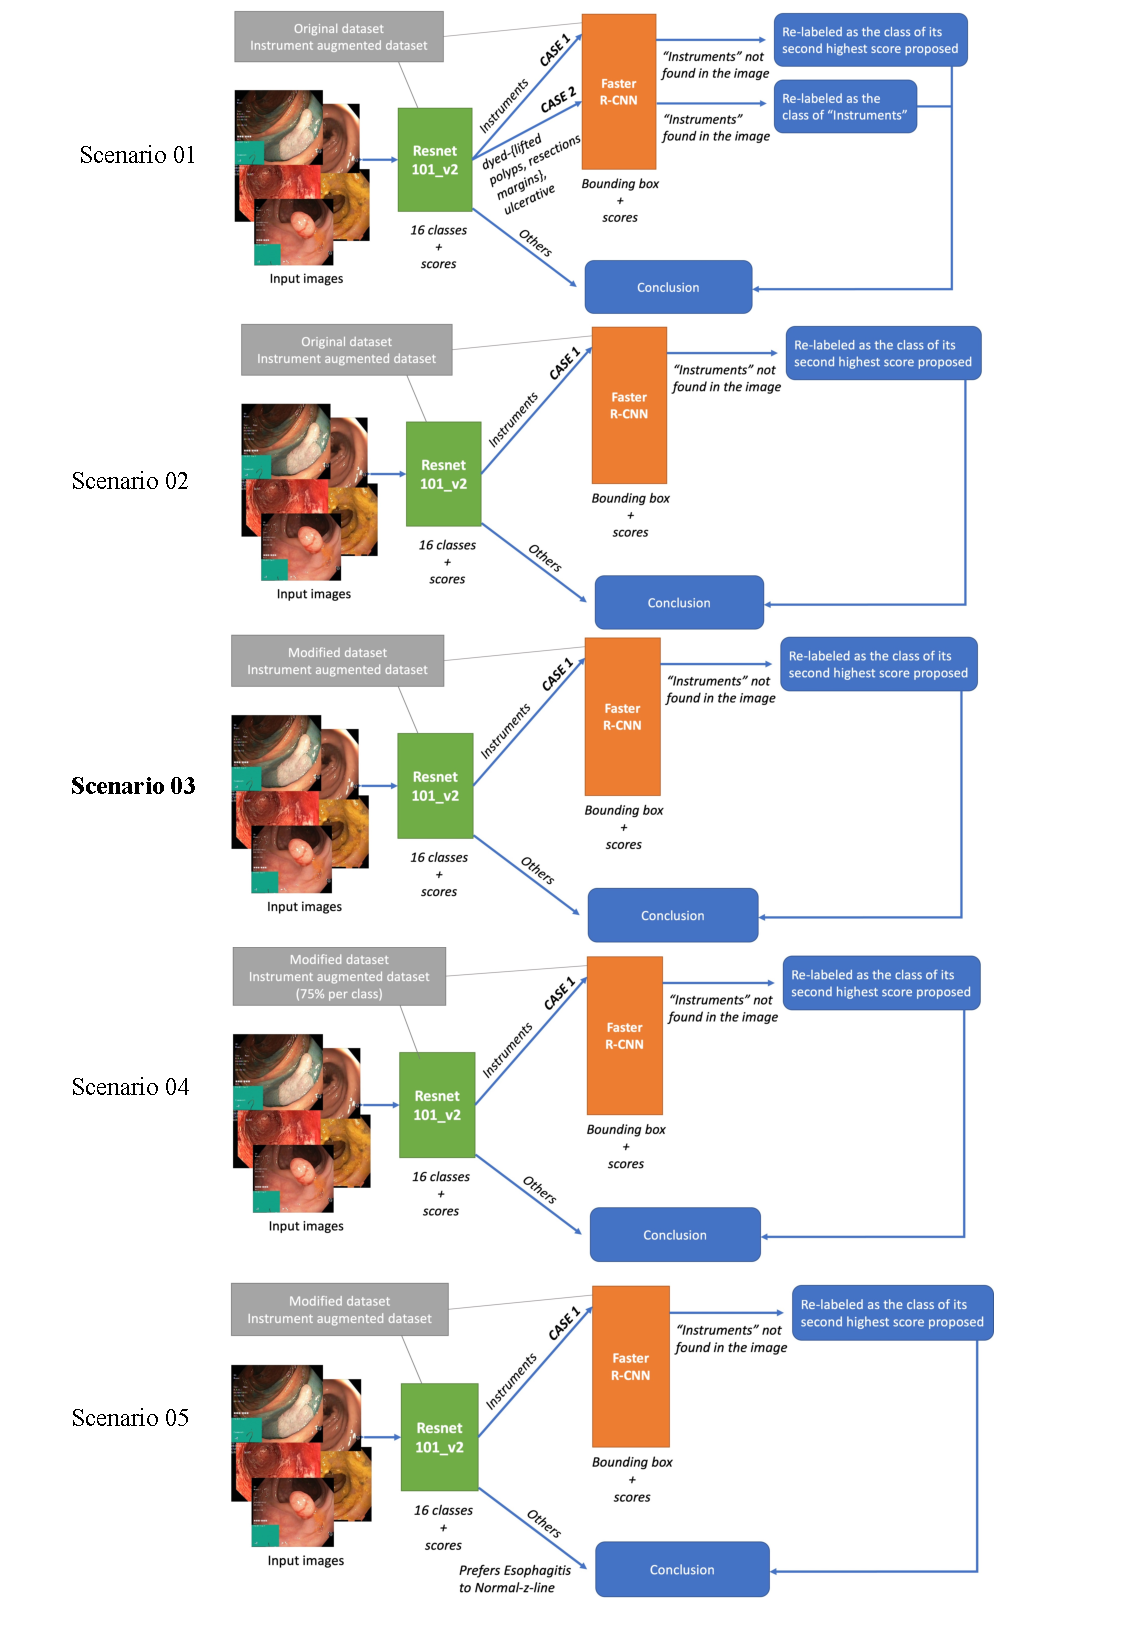
\includegraphics[scale=0.75]{endoscopy_resources/5runs.pdf}
\end{center}
   \caption{Overall process configuration for 5 scenarios.}
\label{fig:5runs}
\end{figure}


As mentioned before, there is a trade-off between the inference time and the accuracy. 
% In Medico 2018, we tried several configurations for our submissions (called \textit{Run}). Totally, we submitted 5 \textit{runs} to organizers. 
The following section describes the pipeline for each of our \textit{runs}. Figure \ref{fig:5runs} illustrates in image. Note that, the \textit{Scenario 03} has performance the best in term of the accuracy while \textit{Scenario 02} has the best inference time. Details and comments about the official evaluate result for each run are further discussed in Section \ref{sec:medico2018_results}.

\subsection{First scenario: \textit{instruments, polyps} double-checked}
Residual network with 101 layers model are fine-tuned on the original development set provided by the task organizers along with our instruments increased dataset. After passed through ResNet101, output images classified as special classes become the input of Faster R-CNN network, which is trained for detecting instruments in images.

\begin{itemize}
    \item First case: Images predicted as \textit{instruments} by Resnet101 are double-checked. In case instruments are not detected by Faster R-CNN in those images, they are re-labeled as the class of their second highest score proposed by Resnet101. %classifier.  
    \item Second case: Images predicted as \textit{dyed-lifted-polyps, dyed-resection-margins, ulcerative colitis} by ResNet101 are fed forward through Faster R-CNN network to detect \textit{instruments}. They are classified as \textit{instruments} if detected or keep the original prediction otherwise.
\end{itemize}

\subsection{Second scenario: \textit{instruments} double-checked}
Feeding forward a large number of images in the three classes through Faster R-CNN causes a bottle-neck of inference time, as Faster R-CNN has high time complexity.
% , around 0.8 second for each image. 
Therefore, in this second , we limited the images passed through Faster R-CNN by only performing the first case of the first scenario.

\subsection{Third scenario: \textit{instruments} double-checked and data augmentation}
The configuration of the third scenario is as same as the second scenario. Instead of using the original training set mentioned in the first scenario, we train our model on the re-labeled development set combined with the augmented instrument set.

\subsection{Forth scenario: 75\% of training set}
In this scenario, we reduce the number of images used for training by selecting randomly 75\% images of each class in the same training set as the third scenario. Other processing steps are also configured in the same way.

\subsection{Fifth scenario: \textit{esophagitis} priority}
Throughout our experiments,
% we realize that the two classes 
\textit{normal-z-line} and \textit{esophagitis} are the top most confusing classes not only for Resnet101 but also for human to distinguish them. In the priority list, \textit{esophagitis} has a higher rank than \textit{normal-z-line's}. Thus, after several times evaluating our model on the development dataset, we propose a condition for these two classes when they are predicted by ResNet101. As ResNet101 provides a probability distribution over the 16 classes for each image, whenever the 
\textit{normal-z-line} appears to be the highest class, we add a small bias $0.3$ to the probability of the \textit{esophagitis}. Hence, the model is more likely to emit the \textit{esophagitis} class. This intuitively means that our model prefers \textit{esophagitis} to \textit{normal-z-line} when it is confused between these classes.

\section{Solving Multi-class Problem with Multi-tasks Classifier}
\label{sec:multi_task}
After Medico 2018, another improvement of our work is to reduce the confusion level of the deep neural network model in cases that various type of abnormalities appeared in a same image. Instead of using only one classifier and forcing the deep neural network model to follow the priority list in these cases by feeding a number  of positive and negative samples, we narrow down this job to multiple classifiers. For instance, given an image that both \textit{esophagitis} and \textit{instruments} appear simultaneously, the job to determine whether or not \textit{instruments} appear inside the image is then left for a 2-classes classifier. This classifier can output the probability that the  given image contains \textit{instruments}. Meanwhile, the  second classifier works independently, which can output the probability for other classes, except \textit{instruments}.

\subsubsection*{Architecture}
In order to reduce the inference time, we decide to share the weights of backbone ResNet 101 for both classifier. The overview of this module can be seen in Figure \ref{fig:multitask_overview}. In general, the proposed multi-task classification model consists of a ResNet 101 architecture except the last fully connected layer, working as a features extractor module that can output a 2048 dimensions vector for  each input image. There are two fully connected branches on top of the output of that features extractor in order to get the prediction of \textit{instruments} class and other 15 \textit{classes}. The number of classifiers is extendable in the future.

\subsubsection*{Loss function}
Two classifiers are trained simultaneously with the overall loss function is a weighted sum of each of their loss, given as follow 
\begin{equation}
       \mathcal{L}(p_i, p_o,p_i^{*},p_o^{*}) = \lambda\sum_{i} \mathcal{L}_{instruments}(p_i, p_i^{*}) + (1-\lambda)\sum_{i}\mathcal{L}_{others}(p_o, p_o^{*})
\end{equation}
where $(p_i,p_i^{*})$ and $(p_o,p_o^{*})$ denote the prediction and the ground-truth of \textit{instruments} class and other classes, respectively. $\mathcal{L}$ is Cross Entropy Loss function. $\lambda$ is a combination weight.

\begin{figure}[H]

\begin{center}
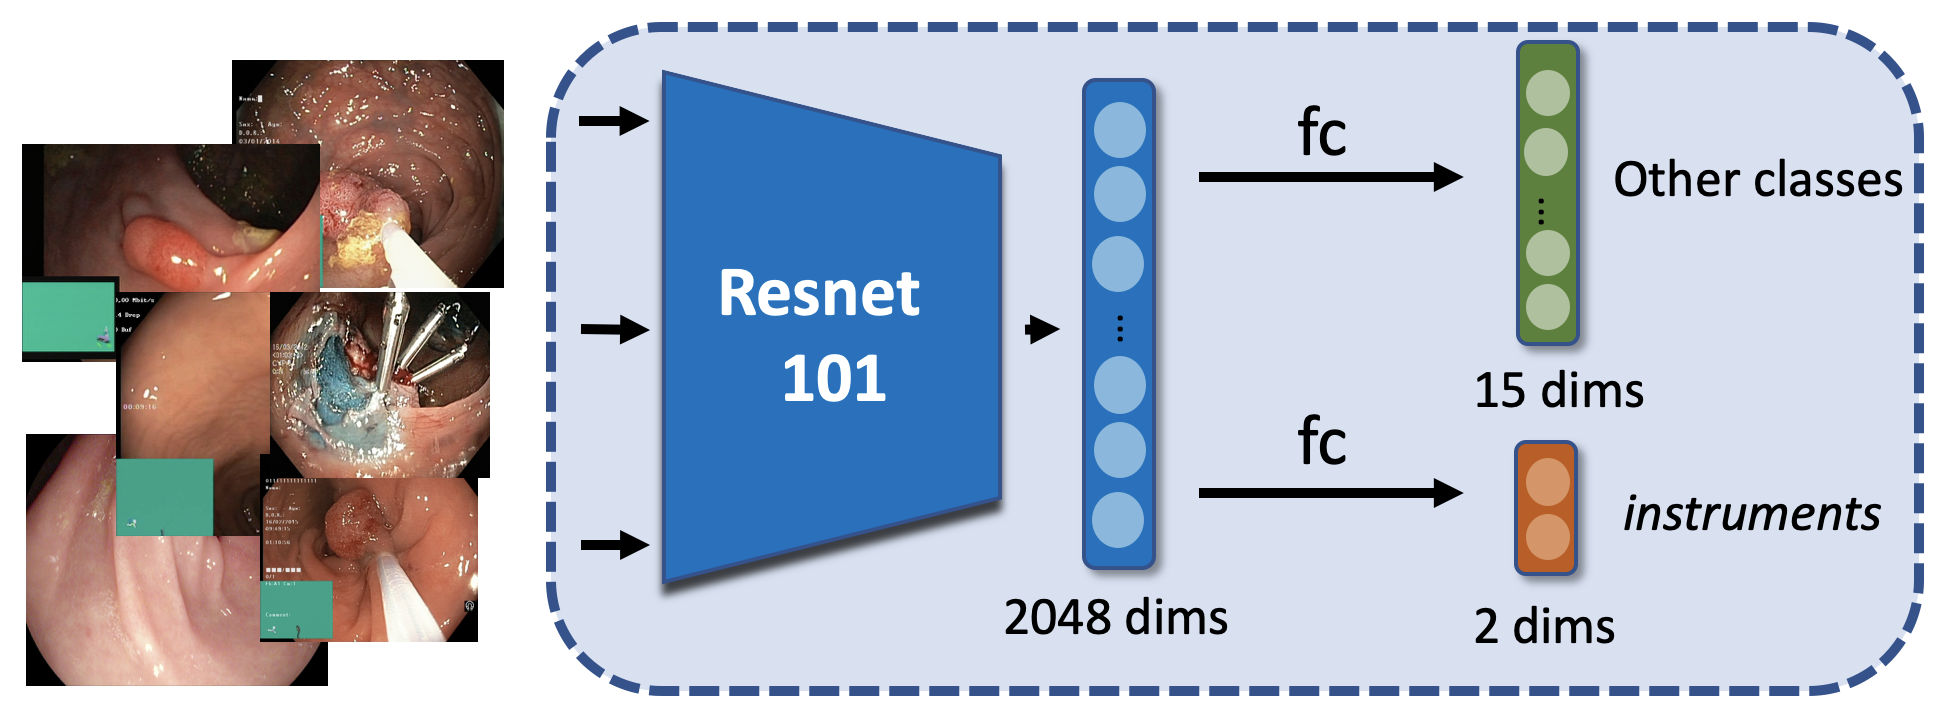
\includegraphics[width=0.8\textwidth]{endoscopy_resources/multi-task.png}
\end{center}
   \caption{Overview of the Multi-class classifier network.}
\label{fig:multitask_overview}
\end{figure}

\subsubsection*{Final prediction}
Since, there are two output vectors from the model, the final prediction can be determined by 

\begin{equation}
    y_{f} = \begin{cases}argmax(p_{o}) & p_{i} < 0.5\\y_{instruments} & p_{i} \geq 0.5\end{cases}
\end{equation}

where $y_{f}$ stands for the final prediction of input image, $p_{o}$ is a 15 dimensions vector indicates the probability that image is likely to belong to. $p_{i}$ is the probability that \textit{instruments} appear inside the image and $y_{instruments}$ is the corresponding label of \textit{instruments} class.

\section{Configuration of Submissions for The Biomedia ACM MM Grand Challenge 2019}
\label{5runs_config}
For the Biomedia ACM MM Grand Challenge 2019 challenge, we continue to tackle existing problems that we did not solve efficiently in Medico 2018, which are the confusing between \textit{normal-z-line} and \textit{esophagitis}; Multi-class problem with \textit{instruments} classes. Besides increasing the size of training data with our augmentation strategy, there are two major improvements in this challenge.
\begin{itemize}
    \item (1) With the Multi-class problem, \textbf{we applied the Multi-tasks Classifier} which is introduced in \ref{sec:multi_task}.
    \item (2) With the \textit{normal-z-line} and \textit{esophagitis}, with a help of a medical expert, we re-annotate the labels of the original dataset and train our models on the modified version of the dataset.
\end{itemize}

In order to evaluate our new improvements to the overall performance of the system, we applied several configurations as given in Table \ref{tab:biomedia_config}.

\begin{table}[h]
\centering
\caption{Experimental configurations for The Biomedia ACM MM Grand Challenge 2019. Character $\bullet$ denotes the corresponding improvement is applied.}
\begin{tabular}{|c|c|c|}
\hline
\multicolumn{1}{|l|}{\textbf{Runs ID}} & \multicolumn{1}{l|}{\textbf{(1)}} & \multicolumn{1}{l|}{\textbf{(2)}} \\ \hline
\textbf{01}                            &                          &                          \\ \hline
\textbf{02}                            & $\bullet$                        &                          \\ \hline
\textbf{03}                            &                          & $\bullet$                        \\ \hline
\textbf{04}                            & $\bullet$                        & $\bullet$                        \\ \hline
\end{tabular}
\label{tab:biomedia_config}
\end{table}

\begin{ChapAbstract}
In this chapter, we discuss the main challenges in applying deep neural network to solve image classification and object detection task on endoscopic image dataset. Especially, we also describe our approaches to overcome mentioned challenges, which can be extend to solve these problems in similar situations.
\end{ChapAbstract}
